\documentclass[xcolor=table,ignorenonframetext,12pt]{beamer}
%\documentclass[xcolor=table,handout,12pt]{beamer}
\usepackage[frenchb]{babel}
\usepackage[utf8]{inputenc}
\usepackage{amsmath,amssymb}
\usepackage{graphicx}
\usepackage{pgfarrows,pgfnodes}
\usepackage{url}
\usepackage{textcomp}
\usepackage[vcentermath]{youngtab}
\usepackage{epstopdf}
\usepackage{hhline}
\usepackage{xmpmulti}
\usepackage{arcs}                       % Pour réaliser le logo TAXIPP
\usepackage{slashbox}                   % Pour réaliser le logo TAXIPP
\usepackage{MnSymbol}                   % Pour réaliser le logo TAXIPP
\PassOptionsToPackage{usenames,dvipsnames,svgnames}{xcolor} % Pour réaliser le logo TAXIPP
\usepackage{xcolor}                     % Pour réaliser le logo TAXIPP
\usepackage{multirow}
\usepackage{subfigure}
\usepackage{booktabs}
\usepackage{tikz}
\usepackage{bbold}
\usepackage{changepage}
\mode<article> {
  \usepackage{fullpage}
  \usepackage{pgf}
  \usepackage{hyperref}
}
\usepackage{tikz}
\usetikzlibrary{shapes.geometric, arrows}
\mode<presentation>
%\usetheme{Madrid}
%\usetheme[left]{Goettingen}
%\setbeamertemplate{background canvas}{\includegraphics[width=\paperwidth]{ippheader.pdf}}
\setbeamertemplate{background canvas}{\hspace{10.1cm}\includegraphics
    [width=0.2\paperwidth]{logo_ipp.pdf}}
\definecolor{ippdark}{RGB}{0,93,116}
\definecolor{ipplight}{RGB}{0,142,156}
\definecolor{ippxlight}{RGB}{0, 204, 204}
\useinnertheme[shadow=true]{rounded}
\setbeamertemplate{items}[circle]
\setbeamercolor{title}{bg=ipplight, fg=black}
\setbeamercolor{structure}{fg=ipplight}
%\setbeamertemplate{sidebar canvas left}{} % pour supprimer le fond de couleur de la barre latérale	
\setbeamertemplate{sidebar canvas left}[vertical shading][top=structure.fg!20,bottom=structure.fg!15]
\setbeamertemplate{caption}[numbered]
\setlength{\leftmargini}{12pt}
\setbeamerfont{framesubtitle}{size=\large}
\definecolor{ippdark}{RGB}{0,93,116}
\definecolor{ipplight}{RGB}{0,142,156}

%\usepackage[latin1]{inputenc}
%\usepackage[english]{babel}

% danger logo
\newcommand*{\TakeFourierOrnament}[1]{{%
\fontencoding{U}\fontfamily{futs}\selectfont\char#1}}
\newcommand*{\danger}{\TakeFourierOrnament{66}}

\newenvironment{checklist}[1]{\begin{list}{$\surd$}{}#1}{\end{list}}%


\newlength{\offsetpage}
\setlength{\offsetpage}{1.0cm}
\newenvironment{widepage}{\begin{adjustwidth}{-\offsetpage}{-\offsetpage}%
		\addtolength{\textwidth}{2\offsetpage}}%
	{\end{adjustwidth}}


% Macro d'inclusion de graphiques pdf %
\newcommand{\graphique}[2][1]{\begin{minipage}{\linewidth}\begin{center}\includegraphics[width=#1\linewidth,clip]{Graphiques/#2}\end{center}\end{minipage}}

\newcommand{\os}[2]{\onslide+<#1->{#2}}%

\newcommand{\m}[2]{\multicolumn{#1}{c}{#2}}%
\newcommand{\ml}[2]{\multicolumn{#1}{l}{#2}}%
\newcommand{\tth}{\textsuperscript{th}}%
\newcommand{\nde}{\textsuperscript{nde}}
\newcommand{\er}{\textsuperscript{er}}
\newcommand{\eme}{\textsuperscript{ème}~}
\newcommand{\hligne}{\begin{tikzpicture}[remember picture,overlay]\node[shift={(-10.5 cm,-1.2cm)}]at(current page.north east){\begin{tikzpicture}{\draw[line width=0.2mm,color=ipplight,overlay](0,0)--(8,0);}\end{tikzpicture}};\end{tikzpicture}\vspace{-0.8cm}}
\newcommand{\hlignee}{\begin{tikzpicture}[remember picture,overlay]\node[shift={(-10.5 cm,-1.2cm)}]at(current page.north east){\begin{tikzpicture}{\draw[line width=0.2mm,color=ipplight,overlay](0,0)--(8,0);}\end{tikzpicture}};\end{tikzpicture}}

% MTABLE: macro for tables %
\newenvironment{mfigure}[4][1]{\def\TMP{#3}\newdimen\TMPsize\settowidth{\TMPsize}{\TMP}
\begin{figure}\caption{#2}\begin{center}\begin{tiny}
\begin{minipage}{#1\textwidth}\resizebox{\textwidth}{!}{#3}\end{minipage}
\if!#4!\empty \else \\
\resizebox{#1\textwidth}{!}{\begin{minipage}{\TMPsize}\begin{tiny}\smallskip\par
#4 \end{tiny}\end{minipage}} \fi}
{\end{tiny}\end{center}\end{figure}}

% Macro pour créer un tableau (avec notes optionnelles) %
\newenvironment{tab}[4][1]
{\def\TMP{#3}\newdimen\TMPsize\settowidth{\TMPsize}{\TMP}
\begin{table}[!ht]
\begin{center}
\begin{minipage}{14cm}
\caption{#2}
\end{minipage}
\end{center}
\begin{center}
\begin{minipage}{#1}
\resizebox{\textwidth}{!}{#3}
\end{minipage}
\if!#4!\empty \else \\
\begin{scriptsize}
\begin{minipage}{#1}\vspace{0.2cm} \par #4
\end{minipage}
\end{scriptsize} \fi }
{\end{center}
\end{table}}

\newenvironment{choixmarges}[2]{\begin{list}{}{%
\setlength{\topsep}{0pt}%
\setlength{\leftmargin}{0pt}%
\setlength{\rightmargin}{0pt}%
\setlength{\listparindent}{\parindent}%
\setlength{\itemindent}{\parindent}%
\setlength{\parsep}{0pt plus 1pt}%
\addtolength{\leftmargin}{#1}%
\addtolength{\rightmargin}{#2}%
}\item }{\end{list}}


\beamertemplatenavigationsymbolsempty


\makeatletter
\def\PENSIPP{PENS\kern-.05em\lower-.19ex\hbox{${\color{BlueGreen} \scalebox{1.4}{\underarc[1]{\overarc[1]{\textcolor{black}{\scalebox{0.7}{ipp}}}}}}\hspace{0.5ex}$}\@}
\makeatother

% numérotation de slides
\setbeamertemplate{footline}[frame number]



\title{Modeling the Careers \\ of the French Public Servants: \\ An Alternative to Wage Equations ?}
\author{ Mahdi Ben Jelloul*, \textbf{Lisa Degalle}* \& Simon Rabaté*}
\institute{
  \inst{*} Institut of Public Policy
}
\subject{}

\setbeamercolor{alerted text}{fg=green}

\date{IMA 6$^{\text{th}}$ World Congress\\
	Torino, June 22nd 2016}

\begin{document}


\frame{\maketitle}




\section{Introduction}


\begin{frame}
\frametitle{Introduction}
\framesubtitle{Modéliser les trajectoires dans les grilles}


\begin{choixmarges}{-0.5cm}{-0.5cm}



\begin{itemize}
\item \textbf{Objectif du module :} modéliser la trajectoire indiciaire des fonctionnaires
\vspace{0.1cm}

\item Approche adoptée: utilisation des grilles de la FPT/FPH

\vspace{0.1cm}
\item Deux processus à modéliser : 
	\begin{enumerate}
	\item Progression au sein d'un grade \\
	\item Changement de grade
	\item[$\Rightarrow$] pour l'instant, focus sur point 2
	\end{enumerate}

\vspace{0.1cm}
\item Deux questions pour le changement de grade : 
	\begin{enumerate}
	\item Quand intervient-il ? 
	\item Vers où ? 
	\item[$\Rightarrow$]  pour l'instant, focus sur point 1
	\end{enumerate}

	
\end{itemize}


\end{choixmarges}
\end{frame}



\begin{frame}
\frametitle{Introduction}
\framesubtitle{Modéliser les trajectoires dans les grilles}

\begin{choixmarges}{-0.5cm}{-0.5cm}
\begin{itemize}
\item \textbf{Objectif du module:} modéliser la trajectoire indiciaire des fonctionnaires.
\vspace{0.1cm}

\item Approche adoptée: utilisation des grilles de la FPT/FPH
	\begin{itemize}
	\item Meilleure simulation des trajectoires salariales
	\item Possibilité de simuler l'impact des réformes des grilles
	\end{itemize}

\vspace{0.1cm}
\item Deux processus à modéliser: 
	\begin{enumerate}
	\item Progression au sein d'un grade \\
	\item Changement de grade
	\item[$\Rightarrow$] pour l'instant, focus sur point 2
	\end{enumerate}

\vspace{0.1cm}
\item Deux questions pour le changement de grade : 
	\begin{enumerate}
	\item Quand intervient-il ? 
	\item Vers où ? 
	\item[$\Rightarrow$]  pour l'instant focus sur point 1 : modélisation de la sortie du grade. 
	\end{enumerate}
\end{itemize}

\end{choixmarges}
\end{frame}


\begin{frame}
\frametitle{Introduction}
\framesubtitle{Résultats présentés}

\begin{choixmarges}{-0.5cm}{-0.5cm}


\begin{itemize}
\item Difficultés rencontrées: 
	\begin{itemize}
	\item Cadre institutionnel: complexe et mouvant
	\item Données: manque de profondeur temporelle 
	\item Econométrie: large censure, effets temporels
	\end{itemize}
 
 \vspace{0.2cm} 
\item Résultats 
	\begin{enumerate}
	\item Procédure d'imputation de la durée passée dans le grade
	\item Preuve de l'effet des contraintes institutionnelles sur les comportements de changement de grade	
		\begin{enumerate}
		\item Analyse graphique
		\item Analyse économétrique (modèle de durée, logit)
		\end{enumerate}
	\item Simulation des sorties de grade sur la base de ces estimations	
		\begin{itemize}
		\item Bon fit global des prédictions
		\item Pas d'amélioration du fit avec l'ajout des variables institutionnelles
		\item Tests pas assez discriminants à ce stade
		\end{itemize}
	 \end{enumerate}
 
	
	\end{itemize}
 

\end{choixmarges}
\end{frame}



\begin{frame}
    \frametitle{Outline of the presentation}
    \tableofcontents[hidesubsections]
\end{frame}





%%%%%%%%% Section 1 -  Background on FPT %%%%%%%%%%%
\section{Institutional background}

\AtBeginSection[]
{
  \begin{frame}[noframenumbering]
    \frametitle{\large Outline}
    \small \tableofcontents[currentsection,hideothersubsections, subsectionstyle=hide]
  \end{frame}
}


%%%%%%%%% Section 2 -  Data %%%%%%%%%%%
\section{Data}

%%%%%%%%% Section 3 -  Graphical evidence %%%%%%%%%%%

\section{Modeling grade changes: relevance of the approach}

\subsection{}

\subsection{Evidence of the impact of institutional conditions}


\begin{frame}

\begin{choixmarges}{-1cm}{-1cm}


\frametitle{Conditions for grade advancement}
\begin{table}
\small
\begin{tabular}{l|c|cc}

\toprule
 Grade  & Type &  \multicolumn{2}{c}{Conditions}  \\
		&  			&  Duration condition	&  Echelon condition \\
\midrule
TTH1  &	Ex. pro. 	&   3y in grade  & 	4  \\
TTH1  &	Au choix 	& 	10y in grade &	7   \\ \midrule
TTH2  & Au choix		& 	6y in corps  &	5   \\ \midrule
TTH3  & Au choix		& 	5y in grade  &	6   \\	
%	
\bottomrule
\end{tabular}
\end{table}
\end{choixmarges}
\end{frame}


\begin{frame}
\frametitle{Graphical evidence for TTH3}
\begin{itemize}
	\item Hazard rate by duration in grade
\end{itemize}
\vspace{-0.2cm}
\begin{center}
\begin{figure}
\includegraphics[width=.75\textwidth]{Graphiques/hazard_by_duree_TTH3.pdf}
\end{figure}
\end{center}
\end{frame}

\begin{frame}
\frametitle{Graphical evidence for TTH3}
\begin{itemize}
	\item Hazard rate by echelon
\end{itemize}
\vspace{-0.2cm}
\begin{center}
\begin{figure}
\includegraphics[width=.75\textwidth]{Graphiques/hazard_by_ech_TTH3.pdf}
\end{figure}
\end{center}

\end{frame}
\begin{frame}
\frametitle{Graphical evidence for TTH3}
\begin{itemize}
	\item Hazard rate by distance to the thresholds
\end{itemize}
\vspace{-0.2cm}
\begin{center}
\begin{figure}
\includegraphics[width=.75\textwidth]{Graphiques/hazard_by_dist_TTH3.pdf}
\end{figure}
\end{center}

\end{frame}


\begin{frame}
\frametitle{Graphical evidence for TTH2}
\begin{itemize}
	\item Hazard rate by duration in grade
\end{itemize}
\vspace{-0.2cm}
\begin{center}
\begin{figure}
\includegraphics[width=.75\textwidth]{Graphiques/hazard_by_duree_TTH2.pdf}
\end{figure}
\end{center}
\end{frame}

\begin{frame}
\frametitle{Graphical evidence for TTH2}
\begin{itemize}
	\item Hazard rate by duration in \textbf{corps}
\end{itemize}
\vspace{-0.2cm}
\begin{center}
\begin{figure}
\includegraphics[width=.75\textwidth]{Graphiques/hazard_by_duree_TTH2_bis.pdf}
\end{figure}
\end{center}
\end{frame}



\begin{frame}
\frametitle{Graphical evidence for TTH2}
\begin{itemize}
	\item Hazard rate by echelon
\end{itemize}
\vspace{-0.2cm}
\begin{center}
\begin{figure}
\includegraphics[width=.75\textwidth]{Graphiques/hazard_by_ech_TTH2.pdf}
\end{figure}
\end{center}
\end{frame}


\begin{frame}
\frametitle{Graphical evidence for TTH2}
\begin{itemize}
	\item Hazard rate by distance to the thresholds
\end{itemize}
\vspace{-0.2cm}
\begin{center}
\begin{figure}
\includegraphics[width=.75\textwidth]{Graphiques/hazard_by_dist_TTH2_bis.pdf}
\end{figure}
\end{center}
\end{frame}


\begin{frame}
\frametitle{Graphical evidence for TTH4}
\begin{itemize}
	\item Hazard rate by duration in grade and echelon
\end{itemize}
\begin{center}
	\includegraphics[width=.5\textwidth]{Graphiques/hazard_by_duree_TTH4.pdf}
	\includegraphics[width=.5\textwidth]{Graphiques/hazard_by_ech_TTH4.pdf}
\end{center}
\end{frame}


\begin{frame}
\frametitle{Graphical evidence for TTH1}
\begin{itemize}
	\item Hazard rate by duration in grade
\end{itemize}
\vspace{-0.2cm}
\begin{center}
\begin{figure}
\includegraphics[width=.75\textwidth]{Graphiques/hazard_by_duree_TTH1.pdf}
\end{figure}
\end{center}
\end{frame}

\begin{frame}
\frametitle{Graphical evidence for TTH1}
\begin{itemize}
	\item Hazard rate by duration from an\_aff
\end{itemize}
\vspace{-0.2cm}
\begin{center}
\begin{figure}
\includegraphics[width=.75\textwidth]{Graphiques/hazard_by_duree_TTH1_bis.pdf}
\end{figure}
\end{center}
\end{frame}



\begin{frame}
\frametitle{Graphical evidence for TTH1}
\begin{itemize}
	\item Hazard rate by echelon
\end{itemize}
\vspace{-0.2cm}
\begin{center}
\begin{figure}
\includegraphics[width=.75\textwidth]{Graphiques/hazard_by_ech_TTH1.pdf}
\end{figure}
\end{center}
\end{frame}


\begin{frame}
\frametitle{Descriptive statistics}
\begin{table}[ht]
	\caption{Number of agents by grade}
	\centering
	\begingroup\footnotesize
	\begin{tabular}{lccccc}
		\hline
		& All & TTH1 & TTH2 & TTH3 & TTH4 \\ 
		\hline
		N & 105110 & 74027 & 15142 & 11667 &  4274 \\ 
		\% & 100 & 70.4 & 14.4 & 11.1 & 4.1 \\ 
		\hline
	\end{tabular}
	\endgroup
\end{table}


\begin{table}[ht]
	\caption{Number of agents by previous grade}
	\centering
	\tiny
	\begingroup\footnotesize
	\begin{tabular}{lcccccc}
		\hline
		& All & Unknown/Left\_censored & Other & TTH1 & TTH2 & TTH3 \\ 
		\hline
		N & 105110 &  8990 & 74993* & 10057 &  7727 &  3343 \\ 
		\% & 100 & 8.6 & 71.3 & 9.6 & 7.4 & 3.2 \\ 
		\hline
	\end{tabular}
\begin{flushleft}
{\footnotesize{\textit{*Among which 61 982 agents have a null wage index (IB)}}}
\end{flushleft}
	\endgroup
\end{table}


\end{frame}
%%%%%%%%% Section 3 -  Duration analysis %%%%%%%%%%%
%\section{Survival analysis}


%\subsection{Censoring}
%
%
%
%\begin{frame}
%\frametitle{Censoring}
%\begin{center}
%\begin{figure}
%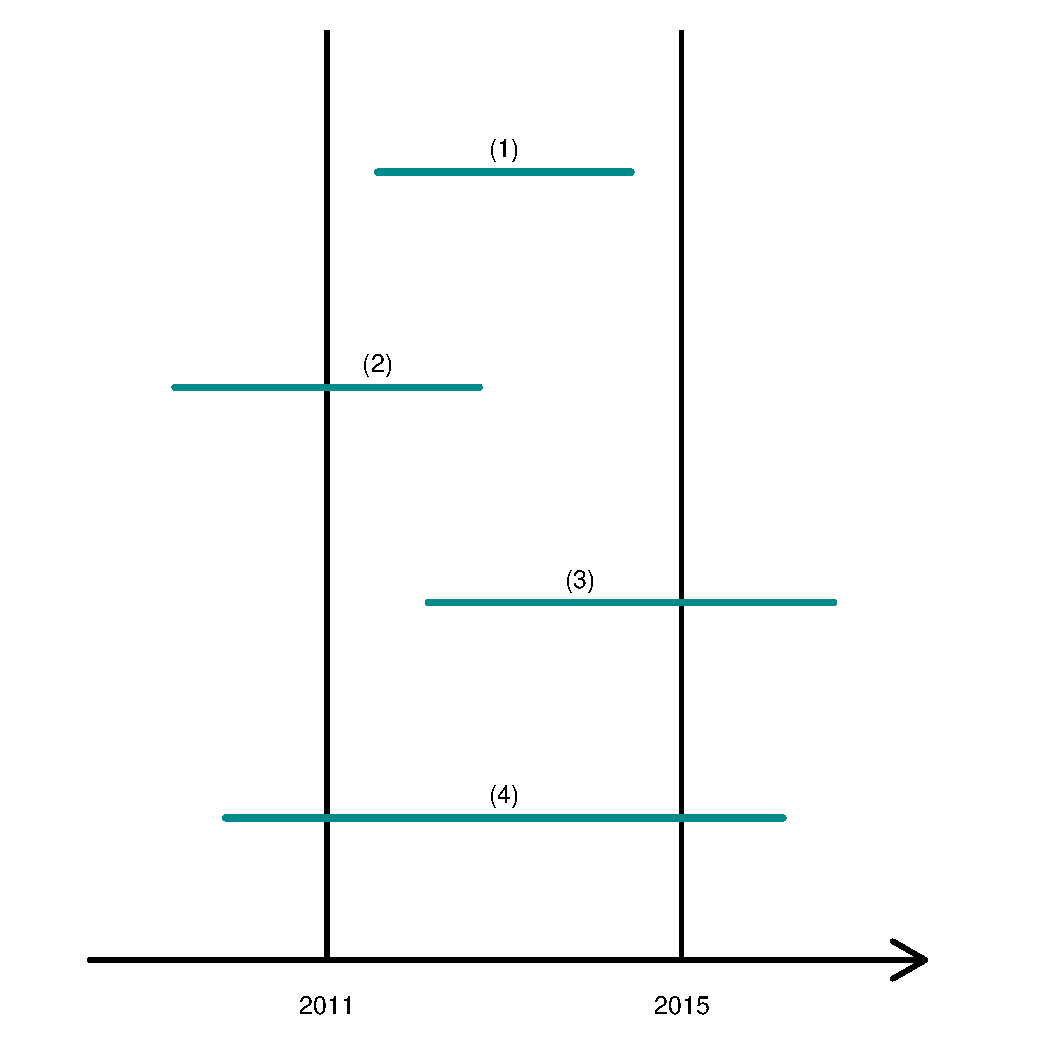
\includegraphics[width=.5\textwidth]{Graphiques/schema_censoring.pdf}
%\end{figure}
%\end{center}
%$\Rightarrow$ Uniquement les cas (2) et (4) ici car 
%
%\begin{table}[ht]
%\centering
%\begingroup\footnotesize
%\begin{tabular}{lccccc}
%  \hline
% & All & TTH1 & TTH2 & TTH3 & TTH4 \\ 
%  \hline
%\% right-censored & 0.567 & 0.670 & 0.198 & 0.320 & 0.757 \\ 
%  \% left-censored & 0.086 & 0.112 & 0.013 & 0.021 & 0.058 \\ 
%   \hline
%\end{tabular}
%\endgroup
%\end{table}
%
%\end{frame}
%
%
%
%\begin{frame}
%\frametitle{Censoring}
%\begin{center}
%\begin{figure}
%
%
%
%
%\end{frame}
%
%
%
%
%\subsection{Estimations}


%%%%%%%%% Section 4 -  Estimation %%%%%%%%%%%
\section{Results}

\subsection{Estimation}


\begin{frame}
\frametitle{Estimation}
\framesubtitle{Duration model}
\begin{choixmarges}{-0.5cm}{-0.5cm}

\begin{itemize}
\item Natural modeling of duration in grade: duration model
	\begin{itemize}
	\item Duration in grade
	\item Handle censoring
	\end{itemize}

\vspace{0.2cm}
\item Several issues encountered: 

\begin{enumerate}
\item Heavy right-censoring (bias)
\item Left truncation (selection of long durations)
\item Difficult to estimate models with time varying and time changing variables (institutionnal conditions). 
\item No baseline hazard from a CoxPH model
\item[] $\Rightarrow$ Problem for simulations. 
\end{enumerate}


\vspace{0.2cm}
\item[$\Rightarrow$] Switch to logit 

\end{itemize}

\end{choixmarges}

\end{frame}



\begin{frame}
\frametitle{Logit estimation}
\framesubtitle{Model}
\begin{choixmarges}{-0.7cm}{-0.7cm}

\small
\begin{equation*}
\begin{array}{c l}
log \frac{P(Change=1)}{1 - P(Change=1)} =& \alpha  + \delta X + \gamma \times duration\_in\_grade + \\
			& \beta_1 \mathbb{1}_{{cond grade 1}} + \beta_2 \mathbb{1}_{{cond ech 1}} +  \beta_3 \mathbb{1}_{{cond grade 1}} \times \mathbb{1}_{{cond ech 2}} +  \\
			& \gamma_0 \mathbb{1}_{{cond grade 2}} + \gamma_1 \mathbb{1}_{{cond ech 1}} + \gamma_3  \mathbb{1}_{{cond grade 2}} \times \mathbb{1}_{{cond ech 2}} 
\end{array} 
\end{equation*}

With :
\vspace{-0.1cm}
\begin{equation*}
\left\{\begin{array}{c  l}
\mathbb{1}_{{cond grade 1}} /\mathbb{1}_{{cond grade 2}}  &= \text{dummy if grade-related conditions are fullfiled}  \\
\mathbb{1}_{{cond ech 1}} / \mathbb{1}_{{cond ech 2}} &= \text{dummy if echelon-related conditions are fullfiled}  \\
X &= \text{gender, generation, grade, year of aff., echelon} \\
 &~~ \text{} 
\end{array} \right.  
\end{equation*}
\normalsize
\vspace{0.1 cm}

\begin{itemize}
\item Sample: all transitions observed between 2011 and 2014.

\end{itemize}

\end{choixmarges}

\end{frame}

\begin{frame}
\frametitle{Logit estimation : \large Results (i)}
\begin{choixmarges}{-0.5cm}{-0.5cm}
\vspace{0.1cm}
\begin{table}
\begin{center}
\scriptsize
\resizebox*{0.9\textwidth}{8.5cm}{\begin{tabular}{l c c c c }
%\toprule
 & Model 1 & Model 2 & Model 3 & Model 4 \\
\midrule
c\_cir\_2011TTH2  & $1.53^{***}$  &               & $1.56^{***}$ & $1.44^{***}$  \\
                  & $(0.01)$      &               & $(0.04)$     & $(0.05)$      \\
c\_cir\_2011TTH3  & $0.91^{***}$  &               & $1.42^{***}$ & $1.29^{***}$  \\
                  & $(0.02)$      &               & $(0.05)$     & $(0.05)$      \\
c\_cir\_2011TTH4  & $-0.26^{***}$ &               & $0.58^{***}$ & $0.47^{***}$  \\
                  & $(0.03)$      &               & $(0.06)$     & $(0.06)$      \\
duration          & $0.24^{***}$  &               &              & $0.10^{***}$  \\
                  & $(0.01)$      &               &              & $(0.01)$      \\
duration2         & $-0.02^{***}$ &               &              & $-0.01^{***}$ \\
                  & $(0.00)$      &               &              & $(0.00)$      \\
I\_echC           &               & $0.25^{***}$  & $0.02$       & $0.02$        \\
                  &               & $(0.02)$      & $(0.02)$     & $(0.02)$      \\
I\_gradeC         &               & $0.11^{***}$  & $-0.02$      & $0.03$        \\
                  &               & $(0.02)$      & $(0.02)$     & $(0.02)$      \\
I\_echE           &               & $-1.06^{***}$ & $0.09$       & $0.07$        \\
                  &               & $(0.05)$      & $(0.06)$     & $(0.06)$      \\
I\_gradeE         &               & $-0.58^{***}$ & $0.42^{***}$ & $0.32^{***}$  \\
                  &               & $(0.03)$      & $(0.05)$     & $(0.05)$      \\
I\_echC:I\_gradeC &               & $1.03^{***}$  & $1.03^{***}$ & $0.97^{***}$  \\
                  &               & $(0.03)$      & $(0.03)$     & $(0.03)$      \\
I\_echE:I\_gradeE &               & $1.16^{***}$  & $0.20^{***}$ & $0.20^{***}$  \\
                  &               & $(0.06)$      & $(0.07)$     & $(0.07)$      \\
\midrule
Controls  		  & Yes  & No    & Yes &  Yes \\
\midrule
AIC               & 227435     & 227090    & 223772    & 223672     \\
Num. obs.         & 315134        & 315134        & 315134       & 315134        \\
\bottomrule
\multicolumn{5}{l}{\scriptsize{$^{***}p<0.01$, $^{**}p<0.05$, $^*p<0.1$}} 
\end{tabular}}
\end{center}
\end{table}


\end{choixmarges}

\end{frame}

\begin{frame}
\frametitle{Logit estimation}
\framesubtitle{Results (ii): interpretation}


\vspace{-0.2cm}

\begin{choixmarges}{-0.7cm}{-0.7cm}

\begin{table}
\centering
\begingroup\footnotesize
\caption{Magnitude of the coefficients for the M4 model}
\vspace{-0.3cm}
\begin{tabular}{lcccccccc}
  \hline
 & Men & 1970s & 1980s & TTH2 & TTH3 & TTH4 & condC & condE \\ 
  \hline
Coeff. & 0.107 & 0.225 & 0.476 & 1.440 & 1.288 & 0.468 & 0.974 & 0.203 \\ 
Odds ratio & 1.113 & 1.252 & 1.609 & 4.223 & 3.626 & 1.597 & 2.649 & 1.226 \\ 
ME & 0.010 & 0.023 & 0.053 & 0.214 & 0.185 & 0.055 & 0.122 & 0.020 \\ 
  Av. ME & 0.011 & 0.024 & 0.055 & 0.211 & 0.181 & 0.056 & 0.124 & 0.021 \\ 
   \hline
\multicolumn{9}{l}{\scriptsize{Ref for generation = 1960s. Ref for grade = TTH1}} \\
\end{tabular}
\endgroup
\end{table}
\end{choixmarges}

\vspace{0.2cm}

Comments
\begin{itemize}
\item  Important effect of the \og au choix \fg{} condition (condC): average increases of the exit probability by 12.4pp (compared to a baseline probility of 13.3pp)
\item  Small than the grade effect, much bigger than the gender effect 
\end{itemize}




\end{frame}

\subsection{Simulation}

\begin{frame}
\frametitle{Adequacy tests}
\framesubtitle{Types of test implemented}
\begin{choixmarges}{-0.5cm}{-0.5cm}


\begin{itemize}

\item MS model: assessment of the quality of the model based on its predictability
\vspace{0.2cm}

\item Ideal test: ability of the model to predict the dynamic of grade exit between 2011 and 2014
	\begin{itemize}
	\item Requires to model the counterfactual echelon evolution for those exiting before 2015
	\item Not done yet
	\end{itemize}
\vspace{0.2cm}

\item Tests used so far: 
	\begin{itemize}
	\item 2011 only: comparison predicted/observed
	\end{itemize}

\end{itemize}
\end{choixmarges}

\end{frame}



\begin{frame}
\frametitle{Adequacy tests}
\framesubtitle{Prediction for year 2011 (i)}
\begin{choixmarges}{-0.5cm}{-0.5cm}

\textbf{Approach}
\begin{enumerate}
\item Split the main sample in two (learning/test samples)
\item Estimate the models on the learning sample 
\item Predict grade exit between 2011 and 2012 from the coefficients in the test sample
\item Compare observed vs. predicted exit
\end{enumerate}
\vspace{0.2cm}

\textbf{Metrics}
\begin{enumerate}
\item Number of exits predicted
\item Proportion of type I and type II errors
\item Effect on key variables: grade and ib 
\end{enumerate}

\end{choixmarges}
\end{frame}



\begin{frame}
\frametitle{Adequacy tests}
\framesubtitle{Prediction for year 2011 (ii)}
\begin{choixmarges}{-0.5cm}{-0.5cm}

\begin{itemize}
\item Estimated models: null model, set 1 of controls, set 1 and 2 of controls and full model
\end{itemize}

\vspace{0.2cm}

\begin{table}[ht]
\centering
\begingroup\footnotesize
\begin{tabular}{lcccc}
  & Model 1 & Model 2 & Model 3 & Model 4 \\ 
  \hline
AIC & 123137 & 114694 & 113237 & 111380 \\ 
  BIC & 123147 & 114774 & 113356 & 111559 \\ 
   \hline
Prop of exit & 0.133 & 0.134 & 0.132 & 0.134 \\ 
  Diff pred. vs. obs & -0.004 & -0.000 & -0.011 & 0.001 \\ 
   \hline
(obs=1 + pred=1)/(obs=1) & 0.136 & 0.193 & 0.198 & 0.215 \\ 
  (obs=1 + pred=0)/(obs=1) & 0.864 & 0.807 & 0.802 & 0.785 \\ 
  (obs=0 + pred=0)/(obs=0) & 0.867 & 0.875 & 0.878 & 0.879 \\ 
  (obs=0 + pred=1)/(obs=0) & 0.133 & 0.125 & 0.122 & 0.121 \\ 
  \end{tabular}
\endgroup
\end{table}


\end{choixmarges}

\end{frame}



\begin{frame}
\frametitle{Adequacy tests}
\framesubtitle{Prediction for year 2011 (iii)}
\begin{choixmarges}{-0.5cm}{-0.5cm}
\begin{table}[ht]
\caption{Proportion of exit by grade, observed vs. predicted}
\centering
\begingroup\footnotesize
\begin{tabular}{lccccc}
  \hline
 & Observed & Model 1 & Model 2 & Model 3 & Model 4 \\ 
  \hline
All & 0.132 & 0.132 & 0.143 & 0.125 & 0.129 \\ 
  TTH1 & 0.079 & 0.132 & 0.088 & 0.075 & 0.082 \\ 
  TTH2 & 0.335 & 0.133 & 0.333 & 0.299 & 0.299 \\ 
  TTH3 & 0.191 & 0.125 & 0.239 & 0.211 & 0.207 \\ 
  TTH4 & 0.089 & 0.135 & 0.063 & 0.046 & 0.054 \\ 
   \hline
\end{tabular}
\endgroup
\end{table}


\end{choixmarges}

\end{frame}


\begin{frame}
\frametitle{Adequacy tests}
\framesubtitle{Prediction for year 2011 (iii)}


\begin{table}[ht]
\centering
\begingroup\footnotesize
\caption{Caracteristics of changing grades individuals}
\begin{tabular}{lccccc}
\toprule
  & Observed & Model 1 & Model 2 & Model 3 & Model 4 \\ 
\midrule
Mean age & 39 & 39 & 39 & 39 & 39 \\ 
\% women & 24 & 30 & 24 & 22 & 23 \\ 
\midrule
\% TTTH1 & 40 & 69 & 42 & 41 & 43 \\ 
\% TTTH2 & 40 & 16 & 36 & 37 & 36 \\ 
\% TTTH3 & 17 & 11 & 20 & 20 & 19 \\ 
\% TTTH4 & 3 & 4 & 2 & 2 & 2 \\ 
\midrule  
  Mean ib & 340 & 329 & 336 & 339 & 338 \\ 
  Q1 ib & 310 & 303 & 310 & 310 & 310 \\ 
  Median ib & 323 & 310 & 323 & 323 & 328 \\ 
  Q3 ib & 360 & 336 & 351 & 360 & 351 \\ 
\bottomrule  
  \end{tabular}
\endgroup
\end{table}


\end{frame}

\section{Conclusion and next steps}


\begin{frame}

\frametitle{Résultats}

\begin{choixmarges}{-0.5cm}{-0.5cm}

\begin{enumerate}
\item Imputation de la durée dans le grade à partir des trajectoires indiciaires
\begin{itemize}
\item Résultats cohérents
\item Suppression de la censure à gauche
\end{itemize}

\vspace{0.2cm}
\item Impact important des conditions institutionnelles ...
\begin{itemize}
\item Statistiques descriptives pour visualiser l'impact des conditions, séparément et en cumulé
\item Effet important dans les estimations
\end{itemize}

\vspace{0.2cm}
\item ... Mais pas d'effets sensibles sur les simulations
\begin{itemize}
\item L'ajout des variables institutionnelles n'améliore pas le fit
\item Surprenant vue la magnitude de l'effet
\item[$\Rightarrow$] Résultat non définitif
\end{itemize}

\end{enumerate}
\end{choixmarges}
\end{frame}



\begin{frame}

\frametitle{Prochaines étapes}

\begin{choixmarges}{-0.5cm}{-0.5cm}

\begin{itemize}

\item A court terme (fin juin/début juillet)

\begin{itemize}

\item Prochaines étapes de modélisation
\begin{itemize}
\item Choix multiples (logit multinomial, emboité?)
\item Modèles de durée
\end{itemize}

\vspace{0.1cm}

\item Améliorer la procédure de test des modèles
\begin{itemize}
\item Sur 2011-2014 (modélisation des échelons)
\item D'autres critères d'évaluations ? 
\end{itemize}

\end{itemize}

\vspace{0.2cm}


\item Questions plus générales:
\begin{itemize}
\item Généralisation des résultats aux autres corps ?
\item Mise en oeuvre dans le modèle
\item Articulation avec les autres modules (affiliation, marché du L)
\end{itemize}

\end{itemize}



\end{choixmarges}
\end{frame}





\section*{Appendix: Completion of career trajectories before 2011}




\subsection{Method}
\begin{frame}
\frametitle{Algorithme}
\begin{itemize}
\item Pour chaque année de 2011 à 2003, pour chaque agent qui n'a pas encore atteint son année d'entrée dans son grade de 2011, on suit cet arbre de décision pour identifier une année d'entrée dans le grade de 2011 :\\
\end{itemize}
\bigskip

\tikzstyle{startstop} = [rectangle, rounded corners, minimum width=0.5cm, minimum height=0.5cm,text centered, draw=black, fill=ipplight]
\tikzstyle{io} = [trapezium, trapezium left angle=70, trapezium right angle=110, minimum width=1cm, minimum height=1cm, text centered, draw=black, fill=ippdark]
\tikzstyle{process} = [rectangle, minimum width=0.5cm, minimum height=0.5cm, text centered, draw=black, fill=ippxlight]
\tikzstyle{decision} = [diamond, minimum width=0.5cm, minimum height=0.5cm, text centered, draw=black, fill=ippdark]
\tikzstyle{arrow} = [thick,->,>=stealth]

\begin{widepage}
\begin{center}
\resizebox{1\textwidth}{3.cm}{
\begin{tikzpicture}[node distance=5cm, sibling distance = 7cm]

\node (start) [startstop, xshift=-3cm, yshift=6cm] {$IB_{t-1}$ sur grille $Grade_{t}$?};
\node (in1) [process, right of=start, xshift=2.5cm] {$Grade_{t}$ = TTH1?}
	child { node {$!\Delta$, $Grade_{t-1}$ = TTH1} edge from parent node[left,draw=none] {oui}}
	child { node (start3) [startstop] {$IB_{t-1}$ sur grille $(Grade-1)_{t}$?} 
		child[yshift=-0.5cm] { node {\begin{tabular}{c} ambigu: \\ !$\Delta$, $Grade_{t-1}$ =  $(Grade-1)_{t}$ ou\\ $\Delta$, $Grade_{t-1}$ =  $(Grade)_{t}$ \end{tabular}} 	edge from parent node[left,draw=none] {oui}}
		child { node {$!\Delta$, $Grade_{t-1}$ = $Grade_{t}$} 	edge from parent node[right,draw=none] {non}}
		edge from parent node[right,draw=none] {non} }
	;

\node (in2) [process, left of=start, xshift=-1.5cm] {$Grade_{t}$ = TTH1?}
child { node {$\Delta$, $Grade_{t-1}$ = autre} edge from parent node[left,draw=none] {oui}}
child { node (start2) [startstop] {$IB_{t-1}$ sur grille $(Grade-1)_{t}$?} 
	child{ node {$\Delta$, $Grade_{t-1}$ = autre} edge from parent node[left, draw=none] {non} }
	child{ node {$\Delta$, $Grade_{t-1}$ = $(Grade-1)_{t}$} edge from parent node[right, draw=none] {oui} }
	edge from parent node[right,draw=none] {non}}
;


\draw [arrow] (start.north) -- node[anchor=north] {oui} (in1.north);
\draw [arrow] (start.north) -- node[anchor=north] {non} (in2.north);

%\draw [arrow] (in1) -- node[anchor=east] {no} (in2);
%
%\draw [arrow] (in2) -- node[anchor=north] {yes} (in1);
%\draw [arrow] (in2) -- node[anchor=east] {no} (in2);
\end{tikzpicture}
}

\end{center}

\end{widepage}
\begin{flushright}
	\hyperlink{chevauchements}{\beamerbutton{Graphique chevauchements}}
\end{flushright}

\end{frame}

\begin{frame}[label = chevauchements]

\frametitle{Appendice : chevauchements de grilles}
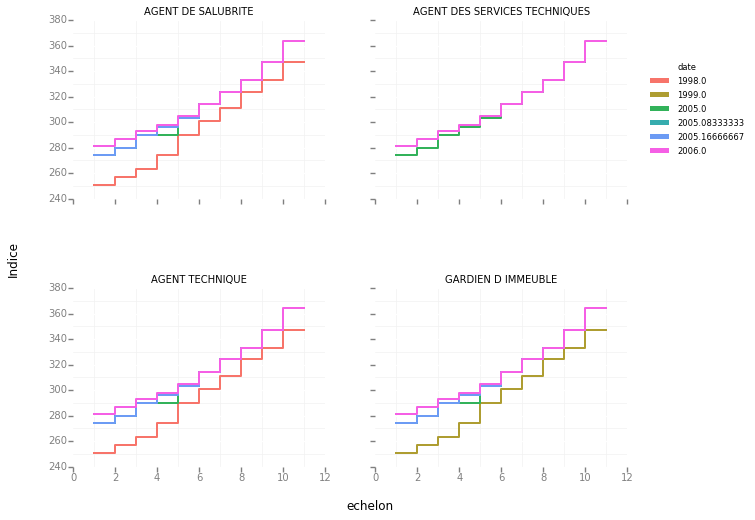
\includegraphics[width=\textwidth]{Graphiques/chevauchements.png}

\end{frame}


\subsection{Results}
\begin{frame}
\frametitle{Résultats}
\begin{itemize}
\item Différence entre l'année d'entrée prédite maximale et d'entrée prédite minimale dans le grade de 2011
\end{itemize}
\begin{figure}
\vspace{-0.5cm}
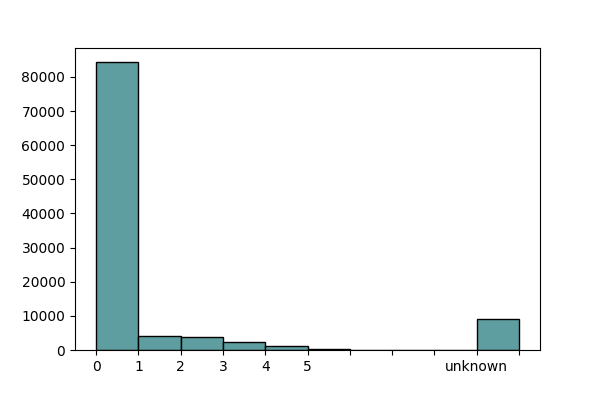
\includegraphics[scale=0.55]{Graphiques/gap.pdf}
\end{figure}

\end{frame}

\begin{frame}
\frametitle{Resultats - suite}
\begin{itemize}
	\item Effectifs par année d'entrée dans le grade de 2011
\end{itemize}
\begin{center}
	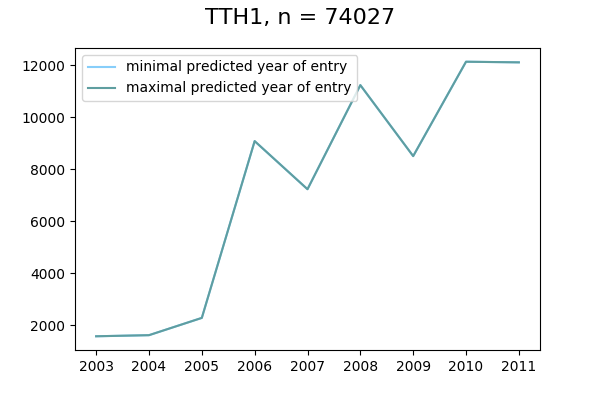
\includegraphics[width=.4\textwidth]{Graphiques/survival_TTH1.pdf}
	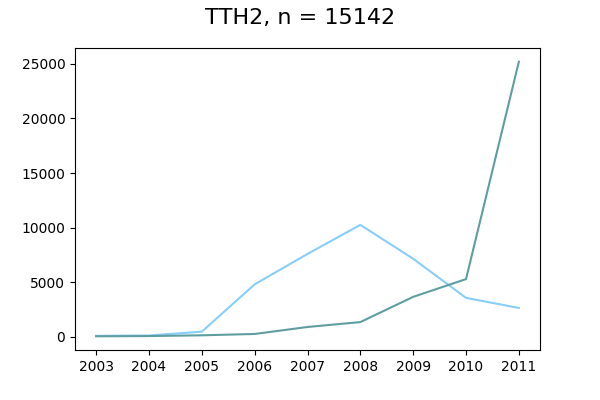
\includegraphics[width=.4\textwidth]{Graphiques/survival_TTH2.pdf}
\end{center}
\begin{center}
	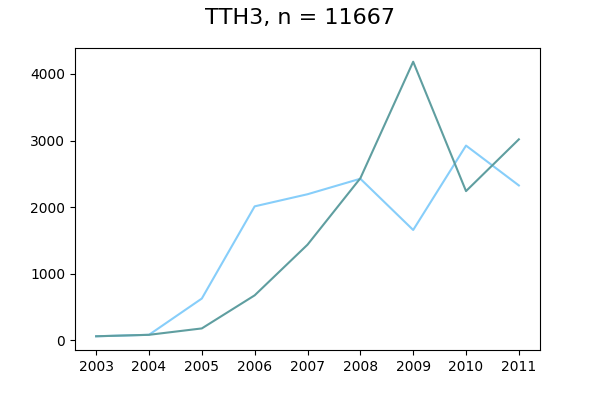
\includegraphics[width=.4\textwidth]{Graphiques/survival_TTH3.pdf}
	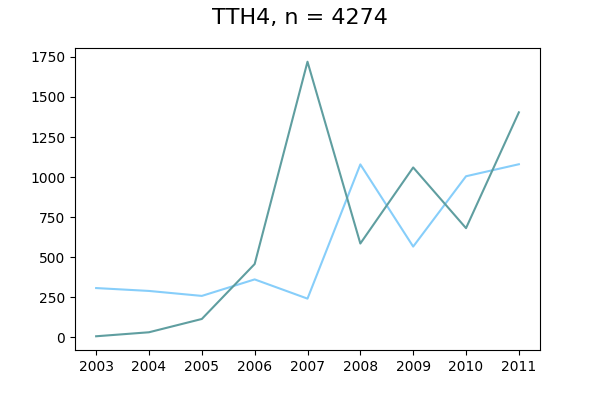
\includegraphics[width=.4\textwidth]{Graphiques/survival_TTH4.pdf}
\end{center}

\end{frame}


\begin{frame}
\frametitle{Resultats - suite}
\begin{itemize}
	\item TTH1
\end{itemize}
\begin{center}
		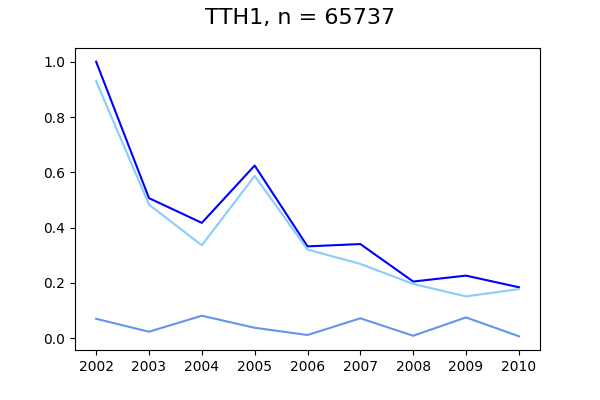
\includegraphics[width=0.55\textwidth]{Graphiques/hazards_TTH1_if_annee_min.pdf}
\end{center}
\begin{center}
		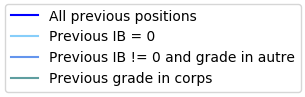
\includegraphics[width=0.3\textwidth]{Graphiques/legend.png}
\end{center}
\end{frame}

\begin{frame}
\frametitle{Resultats - suite}
\begin{itemize}
	\item TTH2
\end{itemize}
	\begin{center}
	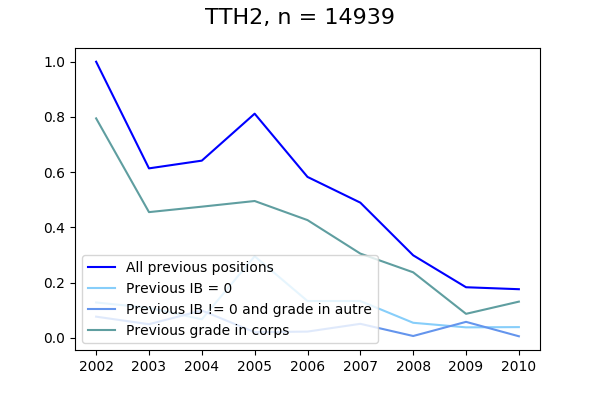
\includegraphics[width=.5\textwidth]{Graphiques/hazards_TTH2_if_annee_min.pdf}
	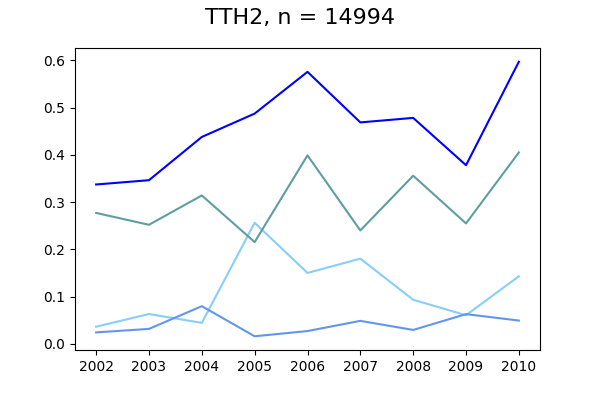
\includegraphics[width=.5\textwidth]{Graphiques/hazards_TTH2_if_annee_max.pdf}
\end{center}
\begin{center}
	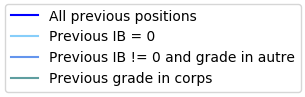
\includegraphics[width=0.3\textwidth]{Graphiques/legend.png}
\end{center}

\end{frame}


\begin{frame}
\frametitle{Resultats - suite}
\begin{itemize}
	\item TTH3
\end{itemize}
\begin{center}
	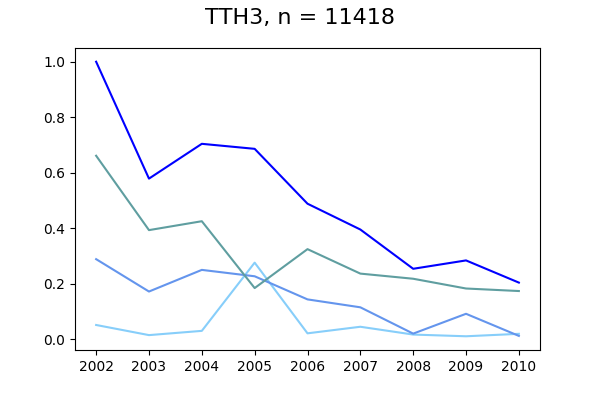
\includegraphics[width=.5\textwidth]{Graphiques/hazards_TTH3_if_annee_min.pdf}
	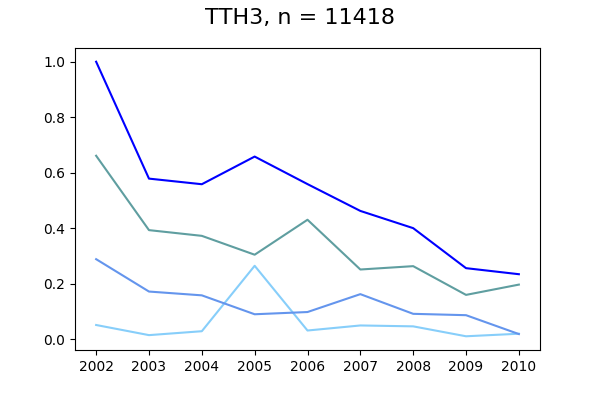
\includegraphics[width=.5\textwidth]{Graphiques/hazards_TTH3_if_annee_max.pdf}
\end{center}
\begin{center}
	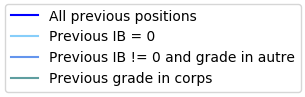
\includegraphics[width=0.3\textwidth]{Graphiques/legend.png}
\end{center}

\end{frame}

\begin{frame}
\frametitle{Resultats - suite}
\begin{itemize}
	\item TTH4
\end{itemize}
\begin{center}
	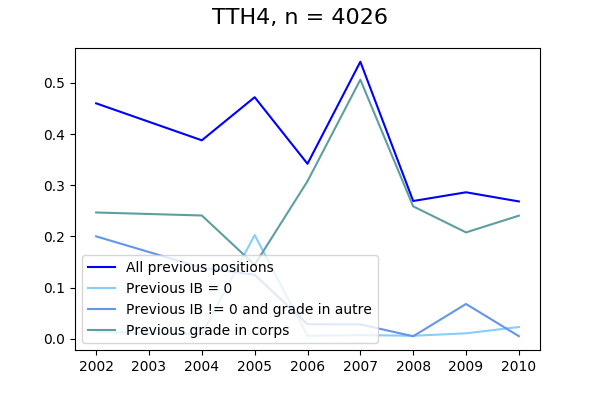
\includegraphics[width=.5\textwidth]{Graphiques/hazards_TTH4_if_annee_min.pdf}
	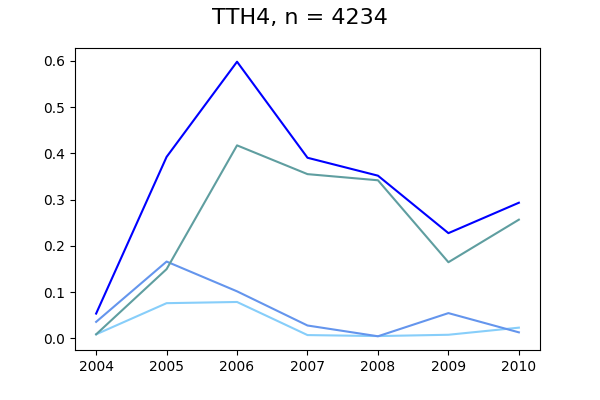
\includegraphics[width=.5\textwidth]{Graphiques/hazards_TTH4_if_annee_max.pdf}
\end{center}
\begin{center}
	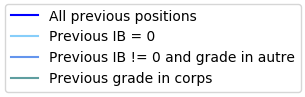
\includegraphics[width=0.3\textwidth]{Graphiques/legend.png}
\end{center}

\end{frame}


\begin{frame}
\frametitle{Comparaison}
\begin{itemize}
	\item Effectifs par année d'affiliation et par grade de 2011
\end{itemize}
\begin{center}
	\includegraphics[width=.5\textwidth]{Graphiques/distrib_an_aff.pdf}
\end{center}


\end{frame}

distrib_an_aff.pdf



\end{document}

% Glossaire
% dépendance: disability
